\section{Introduction:}

A popular area of op-amp application is in instrumentation circuits such as dc or ac voltmeters. A few typical circuits will demonstrate how op-amps can be used.

\subsection{Instrumentation Amplifier:}

A circuit providing an output based on the difference between two inputs (times a scale factor) is shown in Figure 1.1.0. A potentiometer is provided to permit adjusting the scale factor of the circuit. While three op-amps are used, a single-quad op-amp IC is all that is necessary (other than the resistor components). The output voltage can be shown to be: \hfill \break
 
\begin{ceqn}
\begin{align*}
\frac{V_{o}}{V_{1}\ -\ V_{2}}\ =\ 1\ +\ \frac{2R}{R_{p}}.
\end{align*}
\end{ceqn} \hfill \break

so that the output can be obtained from: \hfill \break
 
\begin{ceqn}
\begin{align*}
V_{o}\ =\ (\ 1\ +\ \frac{2R}{R_{p}}\ )\ (\ V_{1}\ -\ V_{2}\ )\ =\ k(\ V_{1}\ -\ V_{2}\ ).
\end{align*}
\end{ceqn} \hfill \break

\begin{figure}[H]
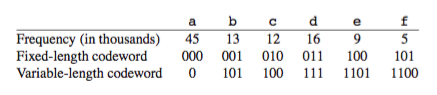
\includegraphics[width = 16.5cm, height = 8cm]{1.png}
\linebreak \linebreak \centering Figure 1.1.0: Instrumentation Amplifier.
\end{figure}

\pagebreak
